\chapter{Application Development}
\label{ch:application-development}

\section{Overview of the Application}

The application is designed to parse textual input that represents a cause-effect graph, converting it into both a visual and logical format. Upon execution, the system performs two key tasks:

\begin{itemize}
    \item \textbf{Graph Visualization}: The first task is to generate a visualized cause-effect graph from the provided textual input. This allows users to clearly see the logical dependencies between causes (inputs) and effects (outputs), facilitating easy analysis of the business logic.
    \item \textbf{Logical Transformation and Decision Table Generation}: In the second phase, the system transforms the cause-effect graph into a logical structure. Through a series of transformation steps, the graph is converted into Boolean logic, and ultimately a decision table is created. This decision table serves as a clear representation of the different logical conditions and their outcomes.
\end{itemize}

All results, including the visual graph, logical transformations, and decision table, are presented in the application's client interface, providing users with an intuitive and comprehensive view of the entire process. The application streamlines the transition from textual cause-effect descriptions to visual models and structured test cases, optimizing the testing workflow for complex systems.

The goal of the application is to simplify and speed up the process of creating cause-effect graphs. Using a textual representation allows for a clearer and more precise definition of the graphs. This approach can effectively represent complex and nested business logic, accommodating various types of rules, causes, and effects.

\section{Technical Overview}

The application is built with a focus on efficiently parsing textual inputs, generating cause-effect graphs, and transforming them into logical structures and decision tables. Below is a detailed technical overview of the key components and technologies used in the development process.

\subsection{Tecnical Stack}

The application is built using a combination of modern technologies, ensuring scalability, maintainability, and ease of development. Below is the breakdown of the technical stack used across various layers of the application.

\subsubsection{Front-End}

For the Front-End, I chose React, a popular JavaScript library, to build the web-based client application. React is a widely adopted library for developing user interfaces, particularly in single-page applications where data dynamically changes without requiring a full page reload.

But why React? React provides a component-based architecture that is highly modular and reusable, making it an excellent choice for building the dynamic and interactive elements of this application. With React, we can efficiently manage and update the user interface as users input data and as the application generates and transforms cause-effect graphs.

React's strength lies in its ability to create highly dynamic user interfaces that are both performant and modular. For this application, which involves continuous interaction and visualization of cause-effect graphs, React is a great fit because of its component-based architecture and ability to efficiently manage frequent updates. However, React does require some upfront learning and the inclusion of third-party libraries for more advanced features. Despite these challenges, its pros make it a robust choice for building scalable and maintainable front-end applications.

React alone wasn't sufficient to construct the application's UI. For the overall styling, I opted for SCSS, which offers a modular and maintainable approach to CSS. Additionally, I integrated Material-UI, a design library that follows Google's Material Design principles.

It's worth highlighting two key libraries that significantly contributed to the functionality of the editor and graph. For the editor, I utilized the Microsoft Monaco Editor, a modern, lightweight, and highly configurable web-based code editor. This tool enhances user experience by providing helpful hints for structuring graphs. For visualizing the graphs, I implemented the Dagre library, which facilitates effective graph rendering.

\subsubsection{Back-End}

For the back-end, I employed Ktor, a Kotlin-based framework designed for building asynchronous servers and web applications. Ktor is known for its flexibility and scalability, allowing developers to create robust APIs with minimal configuration. Its lightweight architecture makes it particularly well-suited for microservices and cloud-native applications. Additionally, Ktor's seamless integration with Kotlin's features, such as coroutines, enhances performance and responsiveness in handling concurrent requests. Overall, Ktor provides an efficient foundation for the back-end of the application, enabling smooth communication between the server and client.

The server's responsibilities include providing initialization data for the client, managing user requests, and executing graph scripts. Kotlin supports its own Domain-Specific Language (DSL) implementation, which I utilized in the future development of the application. This DSL serves as the backbone of the graphing language, allowing for more expressive and concise syntax when defining cause-effect relationships. By leveraging Kotlin's DSL capabilities, I was able to create a more intuitive interface for users to interact with the graphing functionality, enhancing the overall development experience and usability of the application.

For communication, the server is designed to respond via a RESTful API as well as through WebSockets. The RESTful API facilitates standard HTTP requests, enabling seamless interactions between the client and server for data retrieval and manipulation. This allows clients to make synchronous calls for initialization data and other resources.

In addition, the WebSocket implementation provides a persistent connection, enabling real-time communication between the client and server. This is primarily used to provide real-time support for the editor.

Currently, the application does not store any data, so there is no need for a connection to a database or external storage.

\subsubsection{Version Control and CI/CD}

I utilized Git as the version control system throughout the development process, and I employed Microsoft Azure as the remote server for version control.

I also utilized the Microsoft Azure Pipeline feature to automate the deployment process by creating two distinct pipelines.

The first pipeline is dedicated to generating documentation. It produces a PDF document from the source code written in LaTeX format, with the resulting PDF serving as an artifact from this pipeline.

The second pipeline focuses on building and packaging the application. It compiles the back-end using Gradle and the front-end using Yarn. Once the build processes are complete, this pipeline packages the compiled front-end code into the back-end package and designates it as an artifact. Additionally, the artifact is saved into a Docker image and published, streamlining the deployment process further.

\subsubsection{Deployment}

For deployment, I am utilizing Docker with a Linux-based environment. Docker enables the application to be packaged and distributed in a way that ensures it can run independently of the underlying platform. This containerization simplifies the deployment process, allowing the application to maintain consistent behavior across various environments.

Why Docker? Docker is an open-source platform that automates the deployment, scaling, and management of applications within lightweight, portable containers. Each container encapsulates an application along with its dependencies, ensuring that it runs consistently across different computing environments, whether in development, testing, or production. Docker streamlines the application development lifecycle by allowing developers to package their applications in a standardized unit, facilitating easier deployment and scaling while minimizing compatibility issues.

\subsection{Application Architecture}

The architecture of the application is based on a straightforward two-layered model. As the name suggests, the application is divided into two layers: the Front-End and the Back-End. Further details on figure \ref{fig:app-arch}. 

\begin{figure}[H]
	\centering
	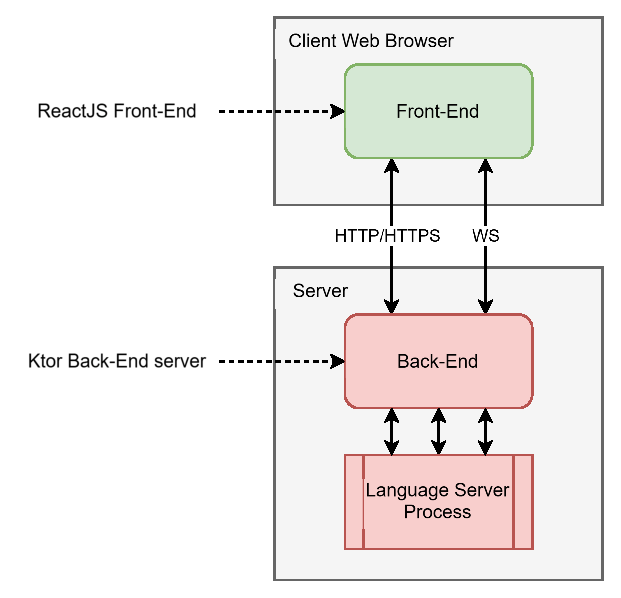
\includegraphics[width=0.5\textwidth,height=240px]{AppArch}
	\caption{Application Architecture}
	\label{fig:app-arch}
\end{figure}

\begin{compactitem}
    \item \textbf{Front-End layer}: This layer is responsible for the user interface and user experience. It handles the presentation of data and interactions with the users, providing a seamless and intuitive interface for creating and managing cause-effect graphs. It is highlighted in green in Figure \ref{fig:app-arch} and operates within the client's web browser.
    \item \textbf{Back-End layer}: This layer manages the application's business logic, data processing, and communication with the front-end. It handles requests from the client, processes them, and sends back the appropriate responses. It is highlighted in red in Figure \ref{fig:app-arch} and operates on a remote server.
\end{compactitem}

\section{Implementation Details}

\section{User Interface}

The user interface of the application is designed to be simple and lightweight. It follows a single-page layout that effectively accommodates the main functionalities. The key features are organized in a tabbed format, with each feature residing in its own dedicated tab. This structure ensures that users can easily navigate between different functionalities without unnecessary complexity, enhancing the overall user experience.

\subsection{Editor}

By default, the \textbf{Editor} tab is selected, and all other tabs are disabled, as there is no valid graph definition present initially. The editor's starting value consists of only an import statement and a graph clause, providing a clean and minimalistic environment for users to begin defining their cause-effect graphs.

Below the editor, there are two buttons. The first button is the \textbf{Reset} button, which restores the editor's content to its initial state, regardless of any edits made. The second button is the \textbf{Execute} button, which is disabled by default. Once the user modifies the content in the editor, the \textbf{Execute} button becomes enabled and is ready for use.

When the \textbf{Execute} button is clicked, the client sends the editor content to the server for evaluation. If the execution encounters any errors, an error message will be displayed, indicating the unsuccessful execution. In other cases, the system will parse the content and define the graph. Once the conversions are complete, the results will activate the other tabs, allowing users to access the newly generated information.

\begin{figure}[H]
	\centering
	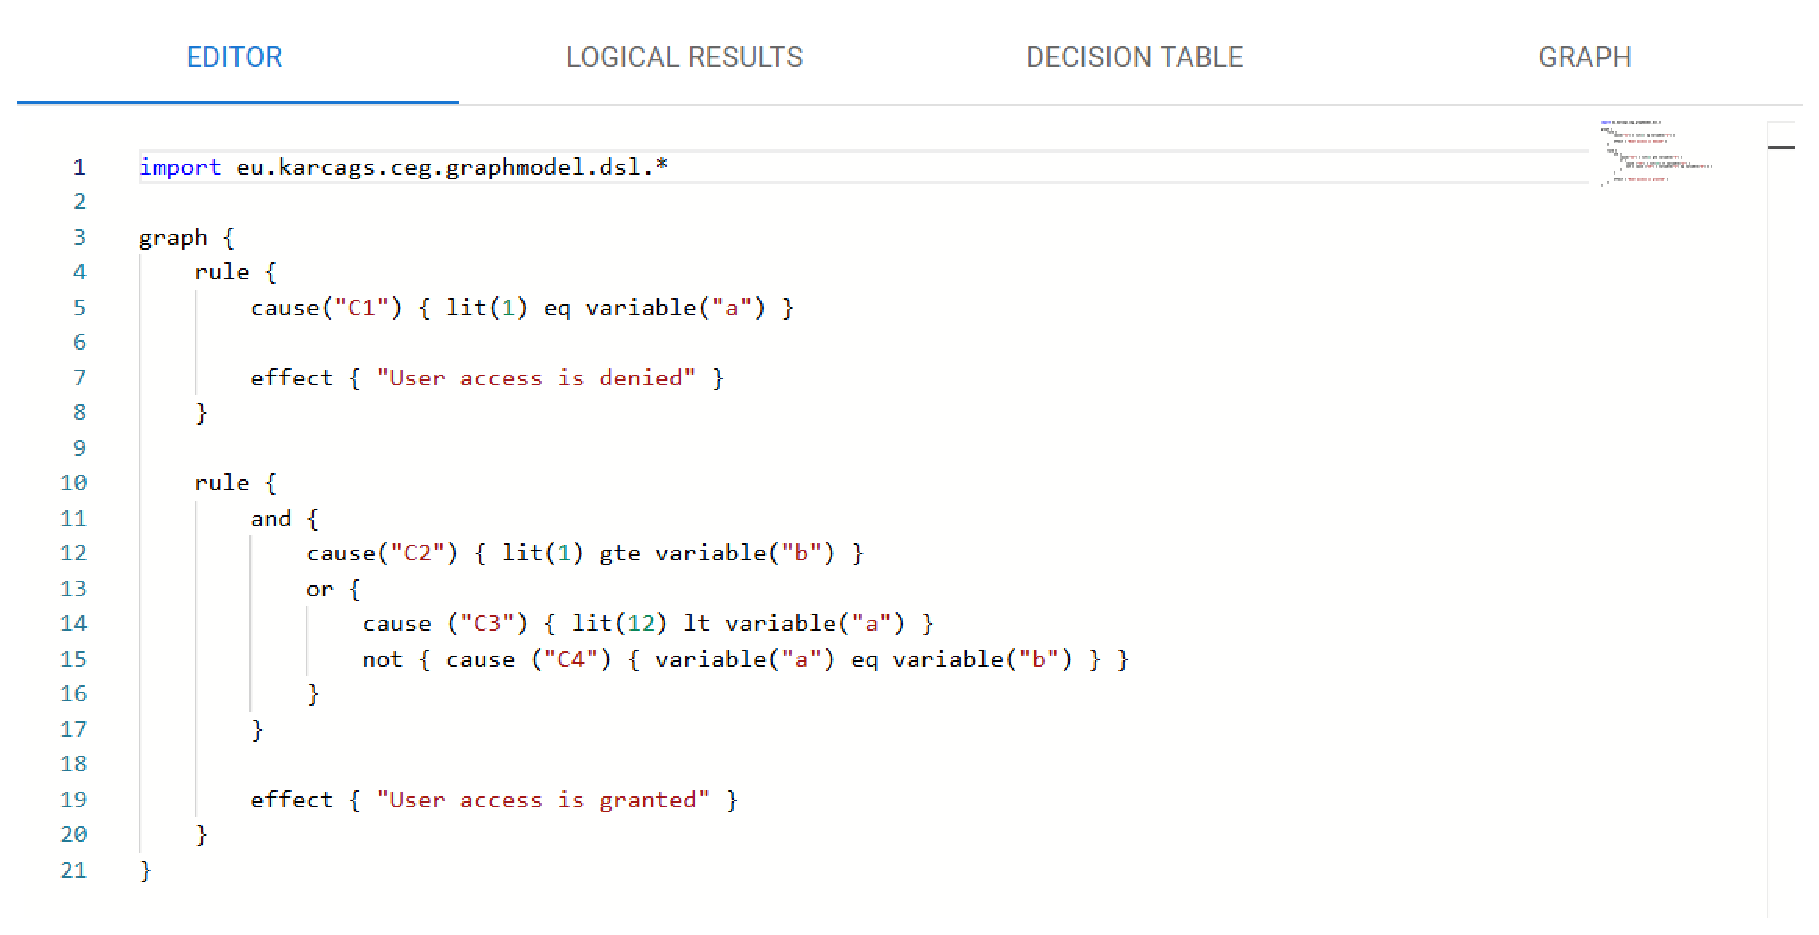
\includegraphics[width=0.8\textwidth,height=160px]{UIEditor}
	\caption{User Interface - Editor tab}
	\label{fig:ui-editor}
\end{figure}

The editor assists users by providing color coding and code IntelliSense features, which include helpful snippets. These enhancements improve the user experience by making it easier to write and understand the graph definitions, reducing the likelihood of errors and streamlining the overall editing process.

\subsection{Logical Results}

After a successful execution, the tabs that depend on the \textbf{Editor} will become available. The \textbf{Logical Results} tab displays the logical formulas parsed from the graph language, along with the corresponding logical formulas after the transformation steps. Each transformation step is presented for each rule, providing a clear overview of the progression from the initial graph to the final logical representation.

\begin{figure}[H]
	\centering
	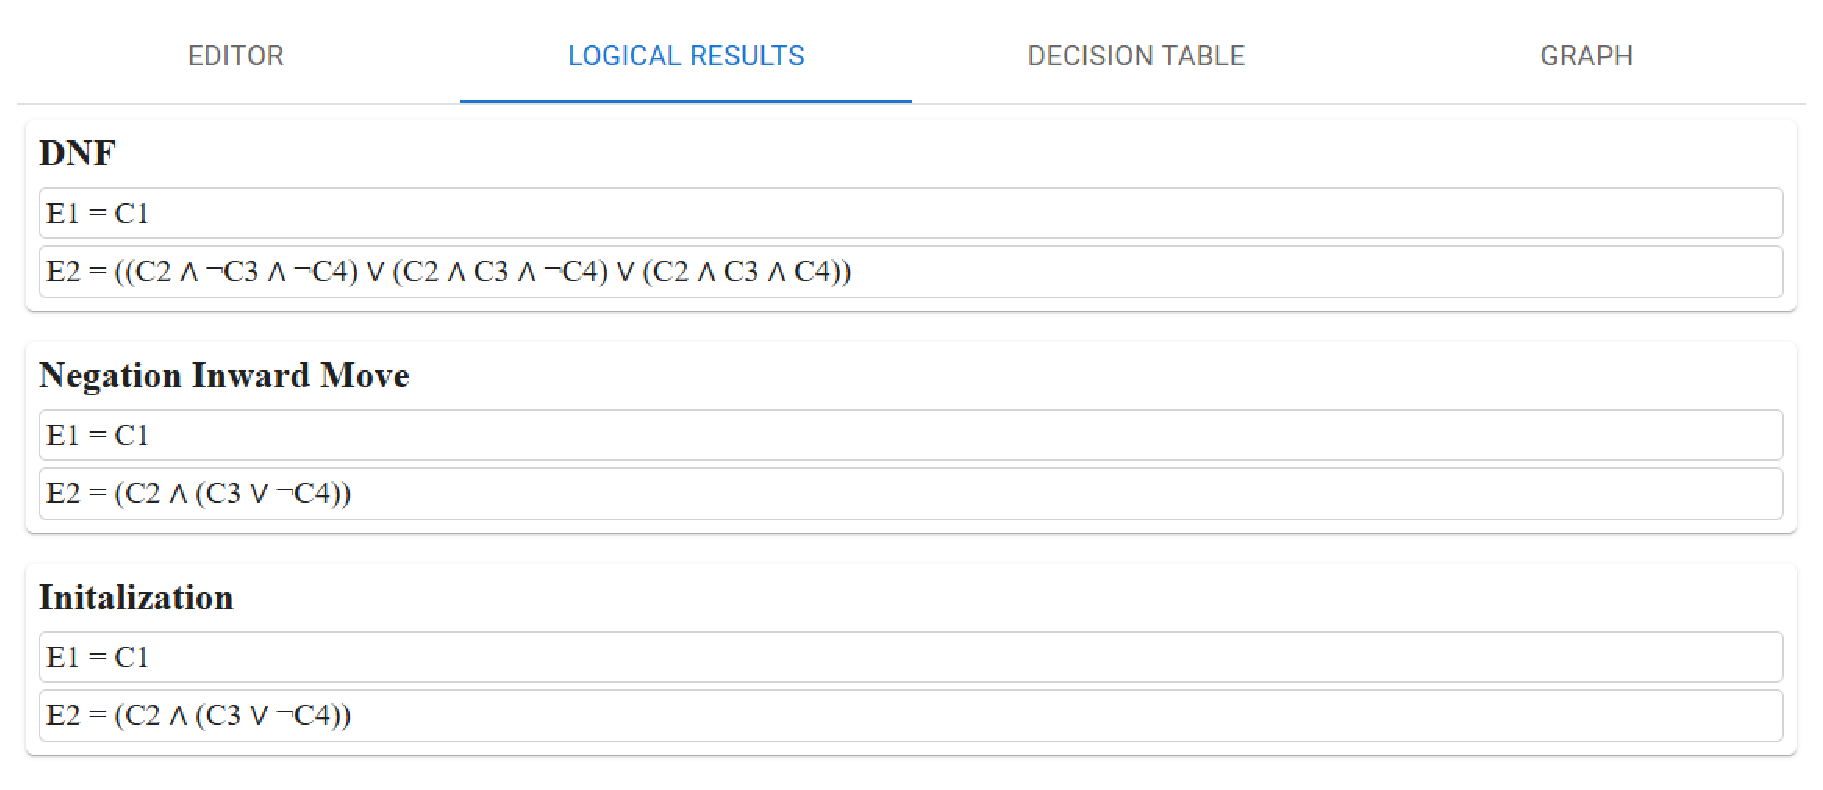
\includegraphics[width=0.8\textwidth,height=160px]{UILogicalResults}
	\caption{User Interface - Logical Results tab}
	\label{fig:ui-logical-results}
\end{figure}

\subsection{Decision Table}

From the final logical results, the system generates a decision table, which is displayed on the third tab. Each rule is converted into one or more columns in the table. Each column collects the causes and their corresponding values necessary to invoke a specific effect, providing a clear and organized representation of the decision-making logic for the further test generation process.

\begin{figure}[H]
	\centering
	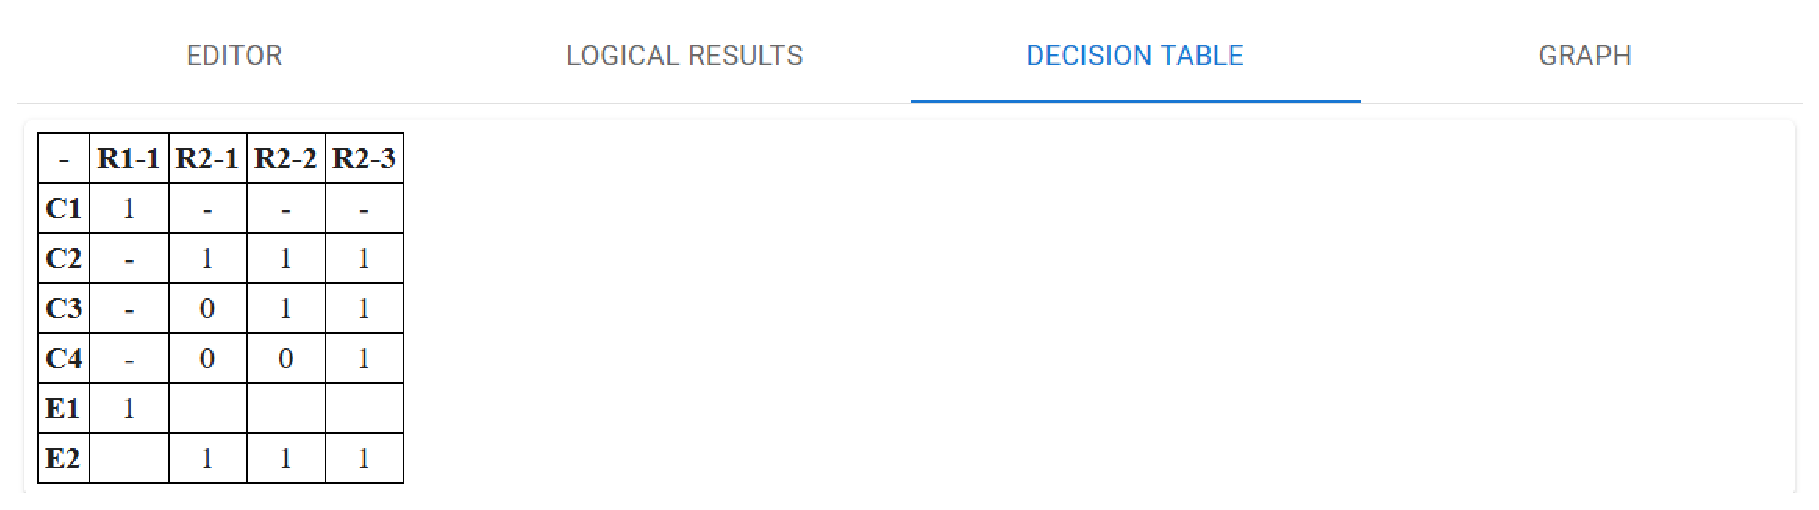
\includegraphics[width=0.8\textwidth,height=120px]{UIDecisionTable}
	\caption{User Interface - Decision Table tab}
	\label{fig:ui-decision-table}
\end{figure}

\subsection{Graph}

On the final tab, a visual representation of the defined graph is displayed. Each node, including causes, effects, and logical nodes, is represented in different colors for easy identification. The nodes are connected to one another by directed arrows, which serve as edges, clearly illustrating the relationships and flow between the various components of the graph.

\begin{figure}[H]
	\centering
	\includegraphics[width=0.8\textwidth,height=280px]{UIGraph}
	\caption{User Interface - Graph tab}
	\label{fig:ui-graph}
\end{figure}

\section{Key Functionalities}